\section{Statistics}
We maintain a {\germinate} statistics page on our server. It shows an overview of all {\germinate} instances that we currently maintain. It's available at:
\begin{center}
	\url{http://ics.hutton.ac.uk/germinate/germinate-statistics}
\end{center}
\noindent
Figure \ref{fig:statistics-overview-table} shows one of the visualizations we provide. We're planning to add more visualizations in the future. Now you might think: "What does that have to do with me?".

The answer is simple: We can add your instance of {\germinate} to our statistics website. That way, people browsing our website may stumble across your site which can broaden your potential target audience. In addition, access to statistical data from more {\germinate} instances allows us to improve {\germinate} and the statistics page. So it's basically a win-win situation.

Just in case you are wondering what kind of data we would collect from your {\germinate} instance, let me go into detail here: When you start {\germinate} on your server, it creates a couple of views. These views contain the aggregated data. You can examine these views with your favourite MySQL tool.

The way we can access this information depends on if your instance of {\germinate} has authentication enabled or not. If not, then there is nothing to do, we can invoke a service on your server using {\germinate}'s API and pull back the aggregated data. If authentication is enabled, you would have to create a new user using {\gatekeeper} and send us the username and password. This user can be a regular user and does not have to be an administrator. We would then store the user credentials in our database and run a query against your views once a day. Consequently, the data we show on our statistics page is always up to date.

If you are interested and want us to add your {\germinate} instance to our statistics page, or if you have any questions, drop us an email: \url{germinate@hutton.ac.uk}.

\begin{figure}
	\centering
	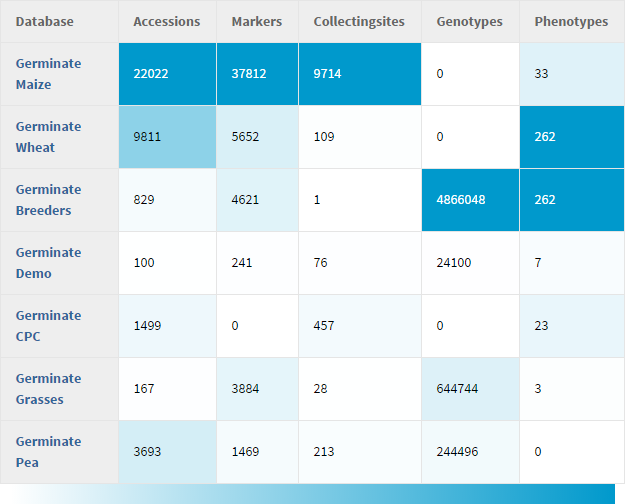
\includegraphics[scale=0.6]{img/statistics/overview-table.png}
	\caption{Statistics overview table}
	\label{fig:statistics-overview-table}
\end{figure}